
%étude de trafic routier



\ifprof
\textit{Corrigé d'après Jérémy Larochette, Lycée Carnot, Dijon, UPS.}
\else
\fi

\ifprof
\else
Ce sujet concerne la conception d'un logiciel d'étude de trafic routier. On modélise le déplacement d'un ensemble de voitures sur des files à sens unique (voir Figure~\ref{ccmp_2017_info_fig_01}). C'est un schéma simple qui peut permettre de comprendre l'apparition d'embouteillages et de concevoir des solutions pour fluidifier le trafic.

Le sujet comporte des questions de programmation. Le langage à utiliser est Python.

\textbf{Notations} :
soit L une liste,
\begin{itemize}
    \item[\textbullet] on note \lstinline{len(L)} sa longueur ;
    \item[\textbullet]  pour $i$ entier, $0 \leqslant  i <$ \lstinline{len(L)}, l'élément de la liste d'indice \lstinline{i} est noté \lstinline{L[i]};
    \item[\textbullet]   pour $i$ et $j$ entiers, $0 \leqslant i < j \leqslant $ \lstinline{len(L)}, $L[i : j]$ est la sous-liste composée des éléments \lstinline{L[i]},
..., \lstinline{L[j - 1]};
    \item[\textbullet]  \lstinline{p*L}, avec \lstinline{p} entier, est la liste obtenue en concaténant \lstinline{p} copies de \lstinline{L}. Par exemple, \lstinline{3*[0]} est
la liste \lstinline{[0, 0, 0]}.
\end{itemize}



%\begin{minipage}{0.45\textwidth}
\begin{center}

%\begin{pspicture}(-2,-2.65)(4,3)
%	\pspolygon(-2,0)(3.5,0)(3.5,0.5)(-2,0.5)%(-2,0)
%    %0.5 pour une case
%    \multido{\nx=-2.0+0.5}{11}{
%    \psline(\nx , 0)(\nx , 0.5)
% }
%\rput(-2,0){\flechemines}
%\rput(-1,0){\flechemines}
%\rput(-0.5,0){\flechemines}
%\rput(3,0){\flechemines}
%\end{pspicture}

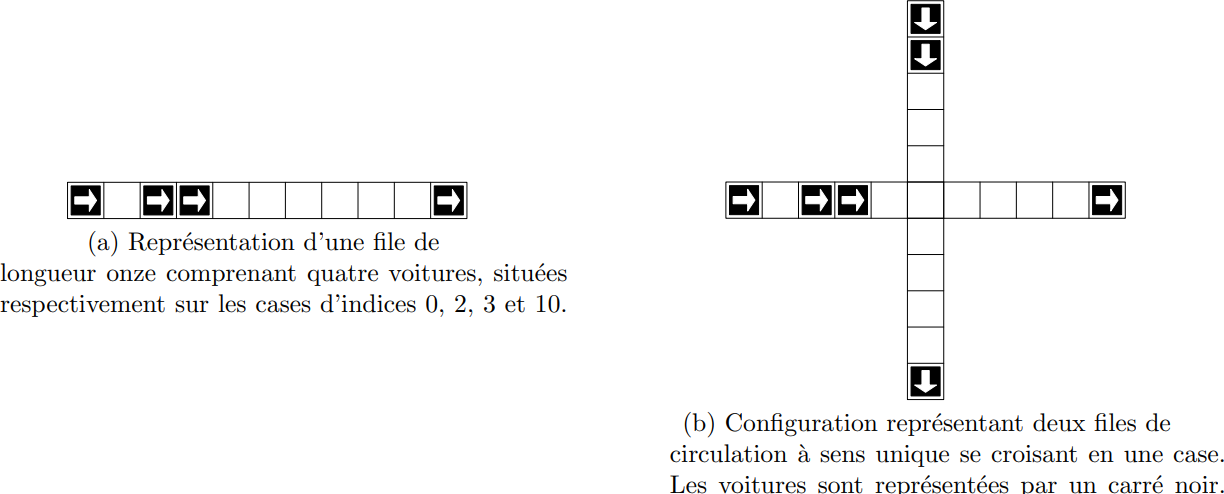
\includegraphics[width=.95\linewidth]{ccmp_2017_info_fig_01}
\captionof{figure}{\label{ccmp_2017_info_fig_01} Files de circulation}
%\captionof{figure}{\label{f_exemple_une_file} Représentation d'une file de longueur onze comprenant quatre voitures, situées respectivement sur les cases d'indices 0, 2, 3 et 10.}
	
\end{center}
%\end{minipage}\hfill
%\begin{minipage}{0.45\textwidth}
%\begin{center}

%\begin{pspicture}(-3.5,-2.65)(3.5,3)
%	\pspolygon(-2.5,0)(3,0)(3,0.5)(-2.5,0.5)%(-2,0)
%    %0.5 pour une case
%    \multido{\nx=-2.5+0.5}{11}{
%    \psline(\nx , 0)(\nx , 0.5)
% }
%\rput(-2.5,0){\flechemines}
%\rput(-1.5,0){\flechemines}
%\rput(-1,0){\flechemines}
%\rput(2.5,0){\flechemines}
%\pspolygon(0,-2.5)(0.5,-2.5)(0.5,3)(0,3)%(-2,0)
%    %0.5 pour une case
%    \multido{\ny=-2.5+0.5}{11}{
%    \psline(0,\ny )(0.5, \ny)
% }
%\rput{-90}(0,2.5){\flechemines}
%\rput{-90}(0,3){\flechemines}
%\rput{-90}(0,-2){\flechemines}
%\end{pspicture}
%\captionof{figure}{\label{f_exemple_deux_file} Configuration représentant deux files de
%circulation à sens unique se croisant en une case.
%Les voitures sont représentées par un carré noir.}
	
%\end{center}
%\end{minipage}
\fi

\section{Préliminaires}



\ifprof
\else
Dans un premier temps, on considère le cas d'une seule file, illustré par la Figure~\ref{ccmp_2017_info_fig_01}(a). Une file de
longueur $n$ est représentée par $n$ cases. Une case peut contenir au plus une voiture. Les voitures
présentes dans une file circulent toutes dans la même direction (sens des indices croissants, désigné
par les flèches sur la Figure~\ref{ccmp_2017_info_fig_01}(a)) et sont indifférenciées.
\fi

\question{Expliquer comment représenter une file de voitures à l'aide d'une liste de booléens.}
\ifprof
\begin{corrige}
Une file de voiture peut \^etre représentée par une liste de booléen : l'élément d'indice $i$ contient \lstinline{True} si et seulement si la case d'indice $i$ contient une voiture.
\end{corrige}
\else
\fi

\question{Donner une ou plusieurs instructions \lstinline{Python} permettant de définir une liste $A$ représentant la file de voitures illustrée par la Figure~\ref{ccmp_2017_info_fig_01}(a).}
\ifprof
\begin{corrige}
 \lstinline{A = [True, False, True, True] + 6 * [False] + [True]}
\end{corrige}
\else
\fi

\question{Soit $L$ une liste représentant une file de longueur $n$ et $i$ un entier tel que $0\leqslant i < n$.
Définir en Python la fonction \lstinline{occupe(L, i)} qui renvoie \lstinline{True} lorsque la case d'indice $i$ de la file est occupée par une voiture et \lstinline{False} sinon.}
\ifprof
\begin{corrige}~\\ \vspace{-.5cm}
\begin{lstlisting}
def occupe(L, i):
    """renvoie True si la case d'indice i de la file représentée par L contient une 
voiture, False sinon."""
    return L[i]
\end{lstlisting}
\end{corrige}
\else
\fi

\question{Combien existe-t-il de files différentes de longueur $n$ ? Justifier votre réponse.}
\ifprof
\begin{corrige}
Chacune des $n$ cases contenant ou non une voiture, il y a exactement $2^n$ files différentes de longueur $n$.
\end{corrige}
\else
\fi

\question{écrire une fonction \lstinline{egal(L1, L2)} retournant un booléen permettant de savoir si deux
listes $L1$ et $L2$ sont égales.}
\ifprof
\begin{corrige} ~\\ \vspace{-.5cm}
\begin{lstlisting} 
def egal(L1, L2):
    "teste si L1 et L2 sont égales"
    if len(L1) != len(L2):
        return False
    for i in range(len(L1)):
        if L1[i] != L2[i]:
            return False
    return True
\end{lstlisting}
\end{corrige}
\else
\fi
%
%\question{Que peut-on dire de la complexité de cette fonction ?}
%\ifprof
%\begin{corrige}
%\end{corrige}
%\else
%\fi

\question{Préciser le type de retour de cette fonction.}
\ifprof
\begin{corrige}
 Cette fonction renvoie un booléen de type \lstinline{bool}.
\end{corrige}
\else
\fi


\section{Déplacement de voitures dans la file}

\ifprof
\else
On identifie désormais une file de voitures à une liste. On considère les schémas de la Figure~\ref{f_etape_simulation_une_file}
représentant des exemples de files. Une étape de simulation pour une file consiste à déplacer les
voitures de la file, à tour de r\^ole, en commen\c cant par la voiture la plus à droite, d'après les règles
suivantes :

\begin{itemize}
	\item  une voiture se trouvant sur la case la plus à droite de la file sort de la file;
    \item  une voiture peut avancer d'une case vers la droite si elle arrive sur une case inoccupée;
    \item  une case libérée par une voiture devient inoccupée;
    \item la case la plus à gauche peut devenir occupée ou non, selon le cas considéré.
\end{itemize}

On suppose avoir écrit en Python la fonction avancer prenant en paramètres une liste de départ,
un booléen indiquant si la case la plus à gauche doit devenir occupée lors de l'étape de simulation,
et renvoyant la liste obtenue par une étape de simulation.


Par exemple, l'application de cette fonction à la liste illustrée par la Figure~\ref{f_etape_simulation_une_file}(a) permet d'obtenir
soit la liste illustrée par la Figure~\ref{f_etape_simulation_une_file}(b) lorsque l'on considère qu'aucune voiture nouvelle n'est
introduite, soit la liste illustrée par la Figure~\ref{f_etape_simulation_une_file}(c) lorsque l'on considère qu'une voiture nouvelle est
introduite.
\fi




%\hfill
%\begin{pspicture}(-7,-2.65)(7,0.65)
%\rput(-0.75,0){%liste initiale, on la centre
%	\pspolygon(-2,0)(3.5,0)(3.5,0.5)(-2,0.5)%(-2,0)
%    %0.5 pour une case
%    \multido{\nx=-2.0+0.5}{11}{
%    \psline(\nx , 0)(\nx , 0.5)
% }
%\rput(-2,0){\flechemines}
%\rput(-1,0){\flechemines}
%\rput(-0.5,0){\flechemines}
%\rput(3,0){\flechemines}
%\uput[-90](0.75,0){(a) Liste initiale \lstinline{A}}
%}%fin (a)
%\rput(-4.75,-2){%liste b
%	\pspolygon(-2,0)(3.5,0)(3.5,0.5)(-2,0.5)%(-2,0)
%    %0.5 pour une case
%    \multido{\nx=-2.0+0.5}{11}{
%    \psline(\nx , 0)(\nx , 0.5)
% }
%\rput(-1.5,0){\flechemines}
%\rput(-0.5,0){\flechemines}
%\rput(0,0){\flechemines}
%%\rput(3,0){\flechemines}
%\uput[-90](0.75,0){(b) \lstinline{B = avancer(A, False)}}
%}%fin liste B
%\rput(3.25,-2){%liste c
%	\pspolygon(-2,0)(3.5,0)(3.5,0.5)(-2,0.5)%(-2,0)
%    %0.5 pour une case
%    \multido{\nx=-2.0+0.5}{11}{
%    \psline(\nx , 0)(\nx , 0.5)
% }
%\rput(-1.5,0){\flechemines}
%\rput(-0.5,0){\flechemines}
%\rput(0,0){\flechemines}
%\rput(-2,0){\flechemines}
%\uput[-90](0.75,0){(c) \lstinline{C = avancer(A, True)}}
%}%fin liste c
%\end{pspicture}
%\hfill {}

\ifprof
\else
\begin{center}
	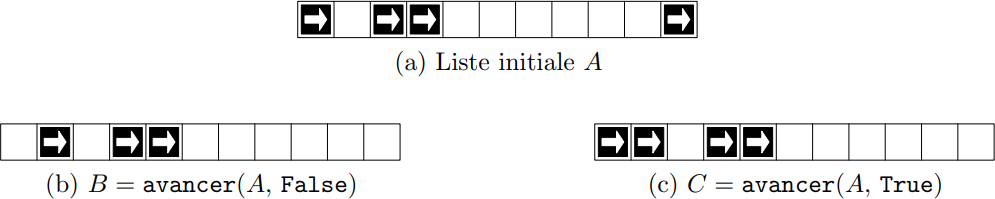
\includegraphics[width=.9\linewidth]{ccmp_2017_info_fig_02}
	\captionof{figure}{\label{f_etape_simulation_une_file}étape de simulation}
\end{center}
\fi

\question{\'Etant donnée $A$ la liste définie à la question~2, que renvoie \lstinline{avancer(avancer(A, False),True)} ?}
\ifprof
\begin{corrige}
\lstinline{[True, False, True, False, True, True, False, False, False, False, False]}.
\end{corrige}
\else
\fi


\ifprof
\else
On considère $L$ une liste et $m$ l'indice d'une case de cette liste ($0 \leqslant m < len(L)$). On
s'intéresse à une étape partielle où seules les voitures situées sur la case d'indice $m$ ou à droite de
cette case peuvent avancer normalement, les autres voitures ne se déplaçant pas.


Par exemple, la file  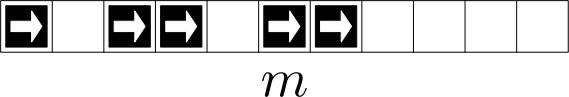
\includegraphics[width=3cm]{ccmp_2017_info_fig_m_01}
%\begin{pspicture}(-3,0)(3,0.5)
%\rput(-0.75,0){%liste initiale, on la centre
%	\pspolygon(-2,0)(3.5,0)(3.5,0.5)(-2,0.5)%(-2,0)
%    %0.5 pour une case
%    \multido{\nx=-2.0+0.5}{11}{
%    \psline(\nx , 0)(\nx , 0.5)
% }
%\rput(-2,0){\flechemines}
%\rput(-1,0){\flechemines}
%\rput(-0.5,0){\flechemines}
%\rput(0.5,0){\flechemines}
%\rput(1,0){\flechemines}
%%\rput(2,0){\flechemines}
%\uput[-90](0.75,0){$m$}
%}%fin (a)
%\end{pspicture}
 devient 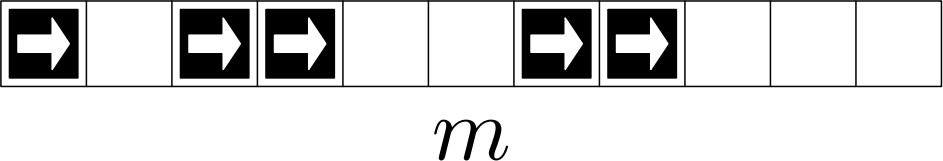
\includegraphics[width=3cm]{ccmp_2017_info_fig_m_02}.
%\begin{pspicture}(-3,0)(3,0.5)
%\rput(-0.75,0){%liste initiale, on la centre
%	\pspolygon(-2,0)(3.5,0)(3.5,0.5)(-2,0.5)%(-2,0)
%    %0.5 pour une case
%    \multido{\nx=-2.0+0.5}{11}{
%    \psline(\nx , 0)(\nx , 0.5)
% }
%\rput(-2,0){\flechemines}
%\rput(-1,0){\flechemines}
%\rput(-0.5,0){\flechemines}
%\rput(1,0){\flechemines}
%\rput(1.5,0){\flechemines}
%\uput[-90](0.75,0){$m$}
%}%fin (a)
%\end{pspicture}



\fi


\question{Définir en Python la fonction \lstinline{avancer_fin(L, m)} qui réalise cette étape partielle de déplacement et renvoie le résultat dans une nouvelle liste sans modifier $L$.}

\ifprof
\begin{corrige}
Version avancer :
\begin{lstlisting}
def avancer_fin(L, m):
    return L[:m] + avancer(L[m:], False)
\end{lstlisting}


Version itérative :
\begin{lstlisting}
def avancer_fin(L, m):
    n = len(L)
    L1 = L[:] # Copie de L
    for i in range(m + 1, n):
        L1[i] = L[i - 1]
    L1[m] = False
    return L1
\end{lstlisting}


Version récursive :
\begin{lstlisting}
def avancer_fin(L, m):
    if m == len(L) - 1:
        L1 = L[:] # Copie de L
        L1[-1] = False
        return L1
    else:
        # Déplacement \`a partir de m + 1
        L1 = avancer_fin(L, m + 1) 
        # Déplacement de m
        L1[m + 1] = L1[m]          
        L1[m] = False
        return L1
\end{lstlisting}
\end{corrige}
\else
\fi

\ifprof
\else
Soient $L$ une liste, $b$ un booléen et $m$ l'indice d'une case inoccupée de cette liste.
On considère une étape partielle où seules les voitures situées à gauche de la case d'indice $m$ se
déplacent, les autres voitures ne se déplacent pas. Le booléen $b$ indique si une nouvelle voiture est
introduite sur la case la plus à gauche.


Par exemple, la file 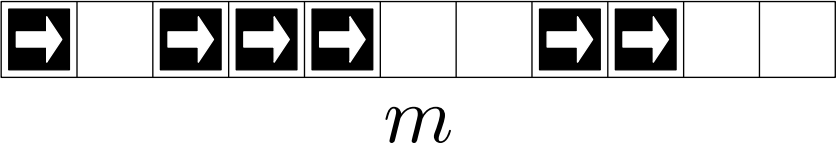
\includegraphics[width=3cm]{ccmp_2017_info_fig_m_03}
%\begin{pspicture}(-3,0)(3,0.5)
%\rput(-0.75,0){%liste initiale, on la centre
%	\pspolygon(-2,0)(3.5,0)(3.5,0.5)(-2,0.5)%(-2,0)
%    %0.5 pour une case
%    \multido{\nx=-2.0+0.5}{11}{
%    \psline(\nx , 0)(\nx , 0.5)
% }
%\rput(-2,0){\flechemines}
%\rput(-1,0){\flechemines}
%\rput(-0.5,0){\flechemines}
%\rput(0,0){\flechemines}
%\rput(1.5,0){\flechemines}
%\rput(2,0){\flechemines}
%\uput[-90](0.75,0){$m$}
%}%fin (a)
%\end{pspicture}
 devient 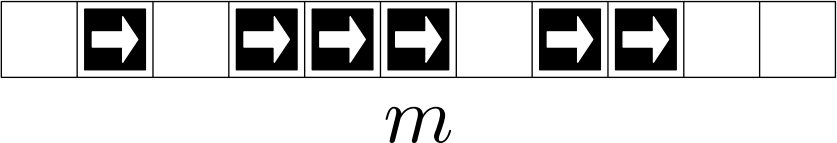
\includegraphics[width=3cm]{ccmp_2017_info_fig_m_04}.
%\begin{pspicture}(-3,0)(3,0.5)
%\rput(-0.75,0){%liste initiale, on la centre
%	\pspolygon(-2,0)(3.5,0)(3.5,0.5)(-2,0.5)%(-2,0)
%    %0.5 pour une case
%    \multido{\nx=-2.0+0.5}{11}{
%    \psline(\nx , 0)(\nx , 0.5)
% }
%\rput(-1.5,0){\flechemines}
%\rput(-0.5,0){\flechemines}
%\rput(0,0){\flechemines}
%\rput(0.5,0){\flechemines}
%\rput(1.5,0){\flechemines}
%\rput(2,0){\flechemines}
%\uput[-90](0.75,0){$m$}
%}%fin (a)
%\end{pspicture}


lorsque aucune nouvelle voiture n'est introduite.

\fi


\question{Définir en Python la fonction \lstinline{avancer_debut(L, b, m)} qui réalise cette étape partielle de déplacement et renvoie le résultat dans une nouvelle liste sans modifier $L$.}
\ifprof
\begin{corrige}
Version avancer :
\begin{lstlisting}
def avancer_debut(L, b, m):
  return avancer(L[:m + 1], b) + L[m + 1:]
\end{lstlisting}

Version itérative :
\begin{lstlisting}
def avancer_debut(L, b, m):
    n = len(L)
    L1 = L[:] # Copie de L
    for i in range(1, m + 1):
        L1[i] = L[i - 1]
    L1[0] = b
    return L1
\end{lstlisting}



Version récursive : 
\begin{lstlisting}
def avancer_debut(L, b, m):
    if m == 1
        L1 = L[:] # Copie de L
        L1[1] = L1[0]
        L1[0] = b
        return L1
    else:
        # Déplacement de m - 1
        L1[m] = L1[m - 1]   
        # Déplacement jusqu'\`a m - 1
        L1 = avancer_debut(L, b, m - 1) 
        return L1
\end{lstlisting}
\end{corrige}
\else
\fi

\ifprof
\else

On considère une liste $L$ dont la case d'indice $m > 0$ est temporairement inaccessible et
bloque l'avancée des voitures. Une voiture située immédiatement à gauche de la case d'indice m ne
peut pas avancer. Les voitures situées sur les cases plus à gauche peuvent avancer, à moins d'être
bloquées par une case occupée, les autres voitures ne se déplacent pas. Un booléen $b$ indique si une
nouvelle voiture est introduite lorsque cela est possible.

Par exemple, la file 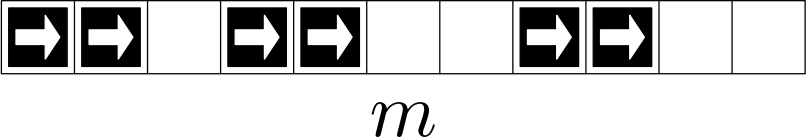
\includegraphics[width=3cm]{ccmp_2017_info_fig_m_05}
%\begin{pspicture}(-3,0)(3,0.5)
%\rput(-0.75,0){%liste initiale, on la centre
%	\pspolygon(-2,0)(3.5,0)(3.5,0.5)(-2,0.5)%(-2,0)
%    %0.5 pour une case
%    \multido{\nx=-2.0+0.5}{11}{
%    \psline(\nx , 0)(\nx , 0.5)
% }
%\rput(-2,0){\flechemines}
%\rput(-1.5,0){\flechemines}
%\rput(-0.5,0){\flechemines}
%\rput(0,0){\flechemines}
%\rput(1.5,0){\flechemines}
%\rput(2,0){\flechemines}
%\uput[-90](0.75,0){$m$}
%}%fin (a)
%\end{pspicture}
 devient 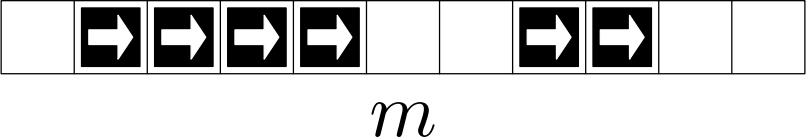
\includegraphics[width=3cm]{ccmp_2017_info_fig_m_06}
%\begin{pspicture}(-3,0)(3,0.5)
%\rput(-0.75,0){%liste initiale, on la centre
%	\pspolygon(-2,0)(3.5,0)(3.5,0.5)(-2,0.5)%(-2,0)
%    %0.5 pour une case
%    \multido{\nx=-2.0+0.5}{11}{
%    \psline(\nx , 0)(\nx , 0.5)
% }
%\rput(-1.5,0){\flechemines}
%\rput(-1,0){\flechemines}
%\rput(-0.5,0){\flechemines}
%\rput(0,0){\flechemines}
%\rput(1.5,0){\flechemines}
%\rput(2,0){\flechemines}
%\uput[-90](0.75,0){$m$}
%}%fin (a)
%\end{pspicture}
%\medskip
lorsque aucune nouvelle voiture n'est introduite.
\fi

\question{Définir en Python la fonction  \lstinline{avancer_debut_bloque(L, b, m)} qui réalise cette étape partielle de déplacement et renvoie le résultat dans une nouvelle liste.}
\ifprof
\begin{corrige}~\\ \vspace{-.5cm}
\begin{lstlisting}
def avancer_debut_bloque(L, b, m):
    L1 = L[:]
    for i in range(m - 1, 0, -1):
        if not occupe(L1, i) \
           and occupe(L1, i - 1): 
            # Voiture en i-1 mais pas en i
            L1[i] = True
            L1[i - 1] = False
    L1[0] = b or L1[0]
    return L1
\end{lstlisting}

\begin{lstlisting}
def avancer_debut_bloque(L, b, m):
    for i in range(m - 1, -1, -1):
        if not occupe(L, i):
            return avancer_debut(L, b, i)
    return L[:]
\end{lstlisting}
\end{corrige}
\else
\fi

\ifprof
\else

On considère dorénavant deux files \lstinline{L1} et \lstinline{L2} de même longueur impaire se croisant en leur
milieu; on note $m$ l'indice de la case du milieu. La file \lstinline{L1} est toujours prioritaire sur la file \lstinline{L2}. Les
voitures ne peuvent pas quitter leur file et la case de croisement ne peut être occupée que par une
seule voiture. Les voitures de la file \lstinline{L2} ne peuvent accéder au croisement que si une voiture de la
file \lstinline{L1} ne s'apprête pas à y accéder. Une étape de simulation à deux files se déroule en deux temps.
Dans un premier temps, on déplace toutes les voitures situées sur le croisement ou après. Dans un
second temps, les voitures situées avant le croisement sont déplacées en respectant la priorité. Par
exemple, partant d'une configuration donnée par la Figure~\ref{f_etapes_simu_deux_files}, les configurations successives sont
données par les Figures~\ref{f_etapes_simu_deux_files}(b), \ref{f_etapes_simu_deux_files}(c), \ref{f_etapes_simu_deux_files}(d), \ref{f_etapes_simu_deux_files}(e) et \ref{f_etapes_simu_deux_files}(f) en considérant qu'aucune nouvelle voiture n'est
introduite.

\fi




\hfill
%\psset{unit = 0.95cm}
%\begin{pspicture}(-8.5,-7)(8.5,7.25)
%\rput(-7,3.5){%(a)
%    \pspolygon(-2.5,0)(3,0)(3,0.5)(-2.5,0.5)%horizontal
%        %0.5 pour une case
%        \multido{\nx=-2.5+0.5}{11}{
%        \psline(\nx , 0)(\nx , 0.5)
%    }
%    \rput(-2.5,0){\flechemines}
%    \rput(-1.5,0){\flechemines}
%    \rput(-1,0){\flechemines}
%    \rput(0,0){\flechemines}
%    \rput(0.5,0){\flechemines}
%    \pspolygon(0,-2.5)(0.5,-2.5)(0.5,3)(0,3)%(vertical
%        %0.5 pour une case
%        \multido{\ny=-2.5+0.5}{11}{
%        \psline(0,\ny )(0.5, \ny)
%    }
%    \rput{-90}(0,3){\flechemines}
%    \rput{-90}(0,2){\flechemines}
%    \rput{-90}(0,1.5){\flechemines}
%    \rput{-90}(0,1){\flechemines}
%    \uput[-90](0.25,-2.5){(a)}
%    \uput[90](0.25,3){L2}
%    \uput[180](-2.5,0.25){L1}
%}%fin (a)
%\rput(0,3.5){%(b)
%    \pspolygon(-2.5,0)(3,0)(3,0.5)(-2.5,0.5)%horizontal
%        %0.5 pour une case
%        \multido{\nx=-2.5+0.5}{11}{
%        \psline(\nx , 0)(\nx , 0.5)
%    }
%    \rput(-2,0){\flechemines}
%    \rput(-1,0){\flechemines}
%    \rput(-0.5,0){\flechemines}
%    \rput(0.5,0){\flechemines}
%    \rput(1,0){\flechemines}
%    \pspolygon(0,-2.5)(0.5,-2.5)(0.5,3)(0,3)%(vertical
%        %0.5 pour une case
%        \multido{\ny=-2.5+0.5}{11}{
%        \psline(0,\ny )(0.5, \ny)
%    }
%    \rput{-90}(0,2.5){\flechemines}
%    \rput{-90}(0,1.5){\flechemines}
%    \rput{-90}(0,1){\flechemines}
%    \rput{-90}(0,0.5){\flechemines}
%    \uput[-90](0.25,-2.5){(b)}
%    \uput[90](0.25,3){L2}
%    \uput[180](-2.5,0.25){L1}
%}%fin b
%\rput(7,3.5){%(c)
%    \pspolygon(-2.5,0)(3,0)(3,0.5)(-2.5,0.5)%horizontal
%        %0.5 pour une case
%        \multido{\nx=-2.5+0.5}{11}{
%        \psline(\nx , 0)(\nx , 0.5)
%    }
%    \rput(-1.5,0){\flechemines}
%    \rput(-0.5,0){\flechemines}
%    \rput(0,0){\flechemines}
%    \rput(1,0){\flechemines}
%    \rput(1.5,0){\flechemines}
%    \pspolygon(0,-2.5)(0.5,-2.5)(0.5,3)(0,3)%(vertical
%        %0.5 pour une case
%        \multido{\ny=-2.5+0.5}{11}{
%        \psline(0,\ny )(0.5, \ny)
%    }
%    \rput{-90}(0,2){\flechemines}
%    \rput{-90}(0,1.5){\flechemines}
%    \rput{-90}(0,1){\flechemines}
%    \rput{-90}(0,0){\flechemines}
%    \uput[-90](0.25,-2.5){(c)}
%    \uput[90](0.25,3){L2}
%    \uput[180](-2.5,0.25){L1}
%}%fin c
%\rput(-7,-3.5){%(d)
%    \pspolygon(-2.5,0)(3,0)(3,0.5)(-2.5,0.5)%horizontal
%        %0.5 pour une case
%        \multido{\nx=-2.5+0.5}{11}{
%        \psline(\nx , 0)(\nx , 0.5)
%    }
%    \rput(-1,0){\flechemines}
%    \rput(0,0){\flechemines}
%    \rput(0.5,0){\flechemines}
%    \rput(1.5,0){\flechemines}
%    \rput(2,0){\flechemines}    
%    \pspolygon(0,-2.5)(0.5,-2.5)(0.5,3)(0,3)%(vertical
%        %0.5 pour une case
%        \multido{\ny=-2.5+0.5}{11}{
%        \psline(0,\ny )(0.5, \ny)
%    }
%    \rput{-90}(0,2){\flechemines}
%    \rput{-90}(0,1.5){\flechemines}
%    \rput{-90}(0,1){\flechemines}
%    \rput{-90}(0,-0.5){\flechemines}
%    \uput[-90](0.25,-2.5){(d)}
%    \uput[90](0.25,3){L2}
%    \uput[180](-2.5,0.25){L1}
%}%fin (d)
%\rput(0,-3.5){%(e)
%    \pspolygon(-2.5,0)(3,0)(3,0.5)(-2.5,0.5)%horizontal
%        %0.5 pour une case
%        \multido{\nx=-2.5+0.5}{11}{
%        \psline(\nx , 0)(\nx , 0.5)
%    }
%    \rput(-0.5,0){\flechemines}
%    \rput(0.5,0){\flechemines}
%    \rput(1,0){\flechemines}
%    \rput(2,0){\flechemines}
%    \rput(2.5,0){\flechemines}    
%    \pspolygon(0,-2.5)(0.5,-2.5)(0.5,3)(0,3)%(vertical
%        %0.5 pour une case
%        \multido{\ny=-2.5+0.5}{11}{
%        \psline(0,\ny )(0.5, \ny)
%    }
%    \rput{-90}(0,1.5){\flechemines}
%    \rput{-90}(0,1){\flechemines}
%    \rput{-90}(0,0.5){\flechemines}
%    \rput{-90}(0,-1){\flechemines}
%    \uput[-90](0.25,-2.5){(e)}
%    \uput[90](0.25,3){L2}
%    \uput[180](-2.5,0.25){L1}
%}%fin e
%\rput(7,-3.5){%(f)
%    \pspolygon(-2.5,0)(3,0)(3,0.5)(-2.5,0.5)%horizontal
%        %0.5 pour une case
%        \multido{\nx=-2.5+0.5}{11}{
%        \psline(\nx , 0)(\nx , 0.5)
%    }
%    \rput(0,0){\flechemines}
%    \rput(1,0){\flechemines}
%    \rput(1.5,0){\flechemines}
%    \rput(2.5,0){\flechemines}
%    %\rput(2.5,0){\flechemines}    
%    \pspolygon(0,-2.5)(0.5,-2.5)(0.5,3)(0,3)%(vertical
%        %0.5 pour une case
%        \multido{\ny=-2.5+0.5}{11}{
%        \psline(0,\ny )(0.5, \ny)
%    }
%    \rput{-90}(0,1.5){\flechemines}
%    \rput{-90}(0,1){\flechemines}
%    \rput{-90}(0,0){\flechemines}
%    \rput{-90}(0,-1.5){\flechemines}
%    \uput[-90](0.25,-2.5){(f)}
%    \uput[90](0.25,3){L2}
%    \uput[180](-2.5,0.25){L1}
%}%fin f
%
%\end{pspicture}\hfill {}

%\psset{unit = 1cm}

\ifprof
\else
\begin{center}
	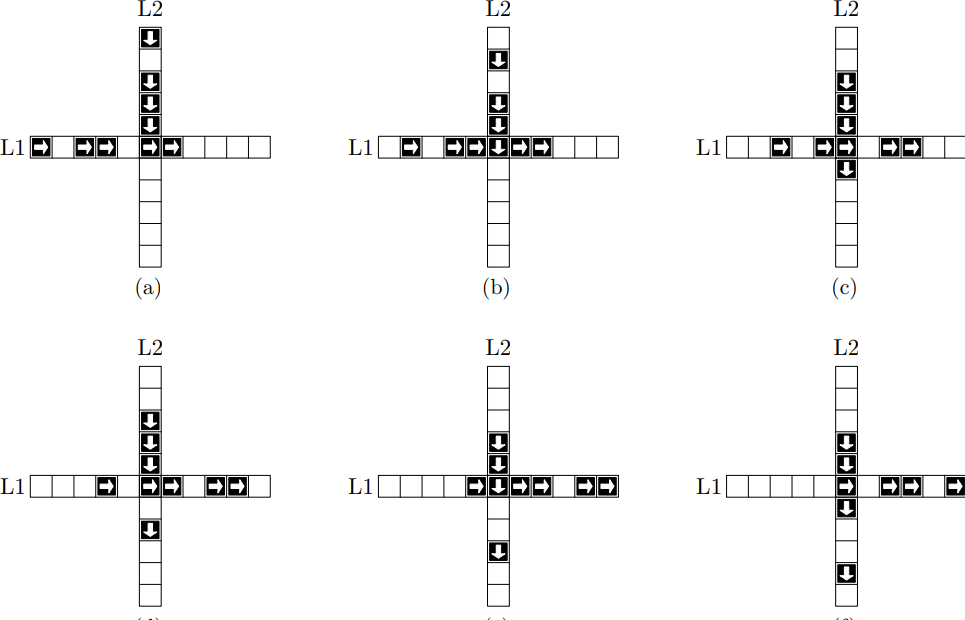
\includegraphics[width=.9\linewidth]{ccmp_2017_info_fig_03}
	\captionof{figure}{\label{f_etapes_simu_deux_files} étapes de simulation à deux files}
\end{center}

\fi


\section{Une étape de simulation à deux files}

\ifprof
\else
L'objectif de cette partie est de définir en \lstinline{Python} l'algorithme permettant d'effectuer une étape
de simulation pour ce système à deux files.
\fi

\question{En utilisant le langage  \lstinline{Python}, définir la fonction  \lstinline{avancer_files(L1, b1, L2, b2)} qui
renvoie le résultat d'une étape de simulation sous la forme d'une liste de deux éléments notée
$[R1, R2]$ sans changer les listes \lstinline{L1} et \lstinline{L2}. Les booléens $b1$ et $b2$ indiquent respectivement si une
nouvelle voiture est introduite dans les files \lstinline{L1} et \lstinline{L2}. Les listes \lstinline{R1} et \lstinline{R2} correspondent aux listes
après déplacement.}

\ifprof
\begin{corrige}~\\ \vspace{-.5cm}
\begin{lstlisting}
def avancer_files(L1, b1, L2, b2):
    m = len(L1) // 2
    R1 = avancer(L1, b1) # Dans tous les cas, L1 avance normalement
    R2 = avancer_fin(L2, m)
    if occupe(R1, m): # une voiture bloque le croisement
        R2 = avancer_debut_bloque(R2, b2, m)
    else:
        R2 = avancer_debut(R2, b2, m)
    return [R1, R2]
\end{lstlisting}
\end{corrige}
\else
\fi


\ifprof
\else
On considère les listes \lstinline{D = [False, True, False, True, False]} et \lstinline{E = [False, True, True, False, False]}
\fi


\question{Que renvoie l'appel  \lstinline{avancer_files(D, False, E, False)} ?}
\ifprof
\begin{corrige}
 L'appel renvoie \lstinline{[[False, False, True, False, True], [False, True, False, True, False]]}.
\end{corrige}
\else
\fi

%
%\section{Transitions}
%
%\question{En considérant que de nouvelles voitures peuvent être introduites sur les premières cases
%des files lors d'une étape de simulation, décrire une situation où une voiture de la file $L2$ serait
%indéfiniment bloquée.}
%
%
%
%\hfill
%%\psset{unit = 0.95cm}
%%\begin{pspicture}(-8.5,-2)(8.5,3.25)
%%\rput(-7,0){%(a)
%%    \pspolygon(-2,0)(2.5,0)(2.5,0.5)(-2,0.5)%horizontal
%%        %0.5 pour une case
%%        \multido{\nx=-2+0.5}{9}{
%%        \psline(\nx , 0)(\nx , 0.5)
%%    }
%%    \rput(-2,0){\flechemines}
%%    \rput(-1.5,0){\flechemines}
%%    \rput(-1,0){\flechemines}
%%    \rput(-0.5,0){\flechemines}
%%    \pspolygon(0,-2)(0.5,-2)(0.5,2.5)(0,2.5)%(vertical
%%        %0.5 pour une case
%%        \multido{\ny=-2+0.5}{9}{
%%        \psline(0,\ny )(0.5, \ny)
%%    }
%%    \rput{-90}(0,1){\flechemines}
%%    \rput{-90}(0,2.5){\flechemines}
%%    \rput{-90}(0,2){\flechemines}
%%    \rput{-90}(0,1.5){\flechemines}
%%    \rput{-90}(0,1){\flechemines}
%%    \uput[-90](0.25,-2){(a)}
%%    \uput[90](0.25,2.5){L2}
%%    \uput[180](-2,0.25){L1}
%%}%fin (a)
%%\rput(0,0){%(b)
%%    \pspolygon(-2,0)(2.5,0)(2.5,0.5)(-2,0.5)%horizontal
%%        %0.5 pour une case
%%        \multido{\nx=-2+0.5}{9}{
%%        \psline(\nx , 0)(\nx , 0.5)
%%    }
%%    \rput(-2,0){\flechemines}
%%    \rput(-1.5,0){\flechemines}
%%    \rput(-1,0){\flechemines}
%%    \rput(-0.5,0){\flechemines}
%%    \pspolygon(0,-2)(0.5,-2)(0.5,2.5)(0,2.5)%(vertical
%%        %0.5 pour une case
%%        \multido{\ny=-2+0.5}{9}{
%%        \psline(0,\ny )(0.5, \ny)
%%    }
%%    \rput{-90}(0,0){\flechemines}
%%    \rput{-90}(0,-0.5){\flechemines}
%%    \rput{-90}(0,-1){\flechemines}
%%    \rput{-90}(0,-1.5){\flechemines}
%%    %\rput{-90}(0,1){\flechemines}
%%    \uput[-90](0.25,-2){(b)}
%%    \uput[90](0.25,2.5){L2}
%%    \uput[180](-2,0.25){L1}
%%}%fin b
%%\rput(7,0){%(c)
%%    \pspolygon(-2,0)(2.5,0)(2.5,0.5)(-2,0.5)%horizontal
%%        %0.5 pour une case
%%        \multido{\nx=-2+0.5}{9}{
%%        \psline(\nx , 0)(\nx , 0.5)
%%    }
%%    \rput(2,0){\flechemines}
%%    \rput(1.5,0){\flechemines}
%%    \rput(1,0){\flechemines}
%%    \rput(0.5,0){\flechemines}
%%    \pspolygon(0,-2)(0.5,-2)(0.5,2.5)(0,2.5)%(vertical
%%        %0.5 pour une case
%%        \multido{\ny=-2+0.5}{9}{
%%        \psline(0,\ny )(0.5, \ny)
%%    }
%%    \rput{-90}(0,0){\flechemines}
%%    \rput{-90}(0,-0.5){\flechemines}
%%    \rput{-90}(0,-1){\flechemines}
%%    \rput{-90}(0,-1.5){\flechemines}
%%    \uput[-90](0.25,-2){(c)}
%%    \uput[90](0.25,2.5){L2}
%%    \uput[180](-2,0.25){L1}
%%}%fin c
%%\end{pspicture}\hfill {}
%
%\begin{center}
%	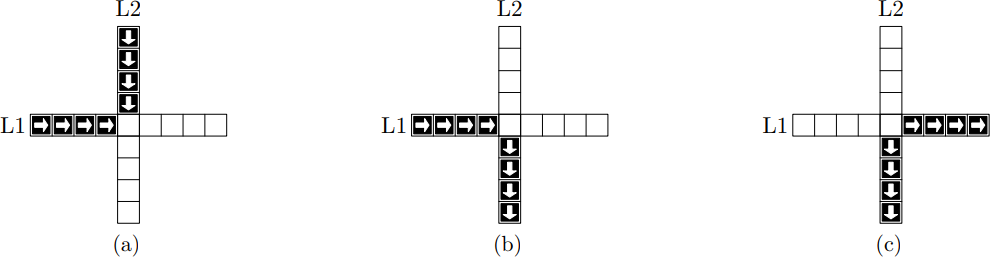
\includegraphics[width=.9\linewidth]{ccmp_2017_info_fig_04}
%	\captionof{figure}{\label{f_etude_config}étude de configurations}
%\end{center}
%
%
%\question{étant données les configurations illustrées par la Figure~\ref{f_etude_config}, combien d'étapes sont nécessaires (on demande le nombre minimum) pour passer de la configuration~\ref{f_etude_config}(a) à la configuration~\ref{f_etude_config}(b)? Justifier votre réponse.}
%
%\question{Peut-on passer de la configuration~\ref{f_etude_config}(a) à la configuration~\ref{f_etude_config}(c)? Justifier votre réponse.}
%
%
%\section{Atteignabilité}
%
%
%Certaines configurations peuvent être néfastes pour la fluidité du trafic. Une fois ces configurations identifiées, il est intéressant de savoir si elles peuvent appara\^\i tre. Lorsque c'est le cas, on dit
%qu'une telle configuration est atteignable.
%Pour savoir si une configuration est atteignable à partir d'une configuration initiale, on a écrit
%le code incomplet donné en annexe.
%Le langage Python sait comparer deux listes de booléens à l'aide de l'opérateur usuel <, on peut
%ainsi utiliser la méthode sort pour trier une liste de listes de booléens.
%
%
%\question{Ecrire en langage Python une fonction \lstinline{elim_double(L)} non récursive, de complexité
%linéaire en la taille de L, qui élimine les éléments apparaissant plusieurs fois dans une liste triée L
%et renvoie la liste triée obtenue. Par exemple \lstinline{elim_double([1, 1, 3, 3, 3, 7])} doit renvoyer la
%liste \lstinline{[1, 3, 7]}.}
%
%
%On dispose de la fonction suivante :
%
%
%\begin{lstlisting}
%def doublons(liste):
%    if len(liste)>1:
%        if liste[0] != liste[1]:
%            return [liste[0]] + doublons(liste[1:])
%        del liste[1]
%        return doublons(liste)
%    else:
%        return liste
%\end{lstlisting}
%
%
%%
%%def doublons(liste):
%%2 if len(liste)>1:
%%3 if liste[0] != liste[1]:
%%4 return [liste[0]] + doublons(liste[1:])
%%5 del liste[1]
%%6 return doublons(liste)
%%7 else:
%%8 return liste
%
%\question{Que retourne l'appel suivant? \lstinline{doublons([1, 1, 2, 2, 3, 3, 3, 5])}}
%
%\question{Cette fonction est-elle utilisable pour éliminer les éléments apparaissant plusieurs fois
%dans une liste non triée? Justifier.}
%
%\question{La fonction recherche donnée en annexe permet d'établir si la configuration correspondant à \lstinline{but} est atteignable en partant de l'état \lstinline{init}. Préciser le type de retour de la fonction \lstinline{recherche}, le type des variables \lstinline{but} et \lstinline{espace}, ainsi que le type de retour de la fonction \lstinline{successeurs}.}
%
%
%\question{Afin d'améliorer l'efficacité du test \lstinline{if but in espace}, ligne 10 de l'annexe, on propose de le remplacer par \lstinline{if in1(but, espace)} ou bien par if \lstinline{in2(but, espace)}, avec \lstinline{in1} et \lstinline{in2} deux fonctions définies ci-dessous. On considère que le paramètre \lstinline{liste} est une liste triée par ordre croissant.
%Quel est le meilleur choix? Justifier.}
%
%
%\begin{lstlisting}
%def in1(element,liste):
%    a = 0
%    b = len(liste)-1
%    while a <= b and element >= liste[a]:
%        if element == liste[a]:
%            return True
%        else:
%            a = a + 1
%    return False
%
%
%def in2(element,liste):
%    a = 0
%    b = len(liste)-1
%    while a < b:
%        pivot = (a+b) // 2 # l'opérateur // est la division entière
%        if liste[pivot] < element:
%            a = pivot + 1
%        else:
%            b = pivot
%    if element == liste[a]:
%        return True
%    else:
%        return False
%\end{lstlisting}
%
%
%
%%def in1(element,liste):
%%2 a = 0
%%3 b = len(liste)-1
%%4 while a <= b and element >= liste[a]:
%%5 if element == liste[a]:
%%6 return True
%%7 else:
%%8 a = a + 1
%%9 return False
%%10
%%11
%%12 def in2(element,liste):
%%13 a = 0
%%14 b = len(liste)-1
%%15 while a < b:
%%16 pivot = (a+b) // 2 # l'opérateur // est la division entière
%%17 if liste[pivot] < element:
%%18 a = pivot + 1
%%19 else:
%%20 b = pivot
%%21 if element == liste[a]:
%%22 return True
%%23 else:
%%24 return False
%
%\begin{enumerate}[label=\ding{111}\textbf{ Q\arabic*} -- ,wide=0pt,resume]
%	\item Afin de comparer plus efficacement les files représentées par des listes de booléens on
%remarque que ces listes représentent un codage binaire où \lstinline{True}correspond à 1 et \lstinline{False} à 0.
%
%écrire la fonction \lstinline{versEntier(L)} prenant une liste de booléens en paramètre et renvoyant l'entier
%correspondant. Par exemple, l'appel \lstinline{versEntier([True, False, False])} renverra 4.
%\item  On veut écrire la fonction inverse de \lstinline{versEntier}, transformant un entier en une liste de
%booléens. Que doit être au minimum la valeur de taille pour que le codage obtenu soit satisfaisant?
%On suppose que la valeur de taille est suffisante. Quelle condition booléenne faut-il écrire en ligne
%4 du code ci-dessous?
%\end{enumerate}
%
%\begin{lstlisting}
%def versFile(n, taille):
%    res = taille * [False]
%    i = taille - 1
%    while ...:
%        if (n % 2) != 0: # % est le reste de la division entière
%            res[i] = True
%        n = n // 2 # // est la division entière
%        i = i - 1
%    return res
%\end{lstlisting}
%
%
%\question{Montrer qu'un appel à la fonction \lstinline{recherche} de l'annexe se termine toujours.}
%
%\question{Compléter la fonction \lstinline{recherche} pour qu'elle indique le nombre minimum d'étapes à
%faire pour passer de \lstinline{init} à \lstinline{but} lorsque cela est possible. Justifier la réponse.}
%
%%
%%\section{ Base de données}
%%
%%On modélise ici un réseau routier par un ensemble de croisements et de voies reliant ces croisements.
%%Les voies partent d'un croisement et arrivent à un autre croisement. Ainsi, pour modéliser une route
%%à double sens, on utilise deux voies circulant en sens opposés.
%%La base de données du réseau routier est constituée des relations suivantes :
%%\begin{itemize}
%%	\item[\textbullet]  Croisement(\underline{id}, longitude, latitude)
%%    \item[\textbullet] Voie(\underline{id}, longueur, id\_croisement\_debut, id\_croisement\_fin)
%%\end{itemize}
%%
%%Dans la suite on considère $c$ l'identifiant (id) d'un croisement donné.
%%
%%\begin{enumerate}[label=\ding{111}\textbf{ Q\arabic*} -- ,wide=0pt,resume]
%%	\item \' Ecrire la requête SQL qui renvoie les identifiants des croisements atteignables en utilisant
%%une seule voie à partir du croisement ayant l'identifiant c.
%%\item écrire la requête SQL qui renvoie les longitudes et latitudes des croisements atteignables
%%en utilisant une seule voie, à partir du croisement c.
%%\item  Que renvoie la requête SQL suivante?
%%\end{enumerate}
%%
%%
%%\begin{lstlisting}{language = SQL}
%%SELECT V2.id_croisement_fin
%%FROM Voie as V1
%%JOIN Voie as V2
%%ON V1.id_croisement_fin = V2.id_croisement_debut
%%WHERE V1.id_croisement_debut = c
%%\end{lstlisting}
%%
%%\newpage
%%
%%\hfill
%% \psshadowbox{\Large Annexe}
%%\hfill {}
%%
%%
%%\begin{lstlisting}
%%def recherche(but, init):
%%    espace = [init]
%%    stop = False
%%    while not stop:
%%        ancien = espace
%%        espace = espace + successeurs(espace)
%%        espace.sort() # permet de trier espace par ordre croissant
%%        espace = elim_double(espace)
%%        stop = egal(ancien,espace) # fonction définie à la question 5
%%        if but in espace:
%%            return True
%%    return False
%%
%%
%%def successeurs(L):
%%    res = []
%%    for x in L:
%%        L1 = x[0]
%%        L2 = x[1]
%%        res.append( avancer_files(L1, False, L2, False) )
%%        res.append( avancer_files(L1, False, L2, True) )
%%        res.append( avancer_files(L1, True, L2, False) )
%%        res.append( avancer_files(L1, True, L2, True) )
%%    return res
%%
%%# dans une liste triée, elim_double enlève les éléments apparaissant plus d'une fois
%%# exemple : elim_double([1, 1, 2, 3, 3]) renvoie [1, 2, 3]
%%def elim_double(L):
%%# code à compléter
%%
%%# exemple d'utilisation
%%# debut et fin sont des listes composées de deux files de même longueur impaire,
%%# la première étant prioritaire par rapport à la seconde
%%debut = [5*[False], 5*[False]]
%%fin = [3*[False]+2*[True], 3*[False]+2*[True]]
%%print(recherche(fin,debut))
%%\end{lstlisting}
%%
%%\hfill
%% \psshadowbox{\Large Fin de l'épreuve.}
%%\hfill {}
%%
%%\label{LastPage}
%%\end{document}